\chapter{Attachments}

\section{AVS Tasks at VBS 2018}\label{att:vbs_tasks_timeline_avs}

\begin{figure}[h]
	\centering
	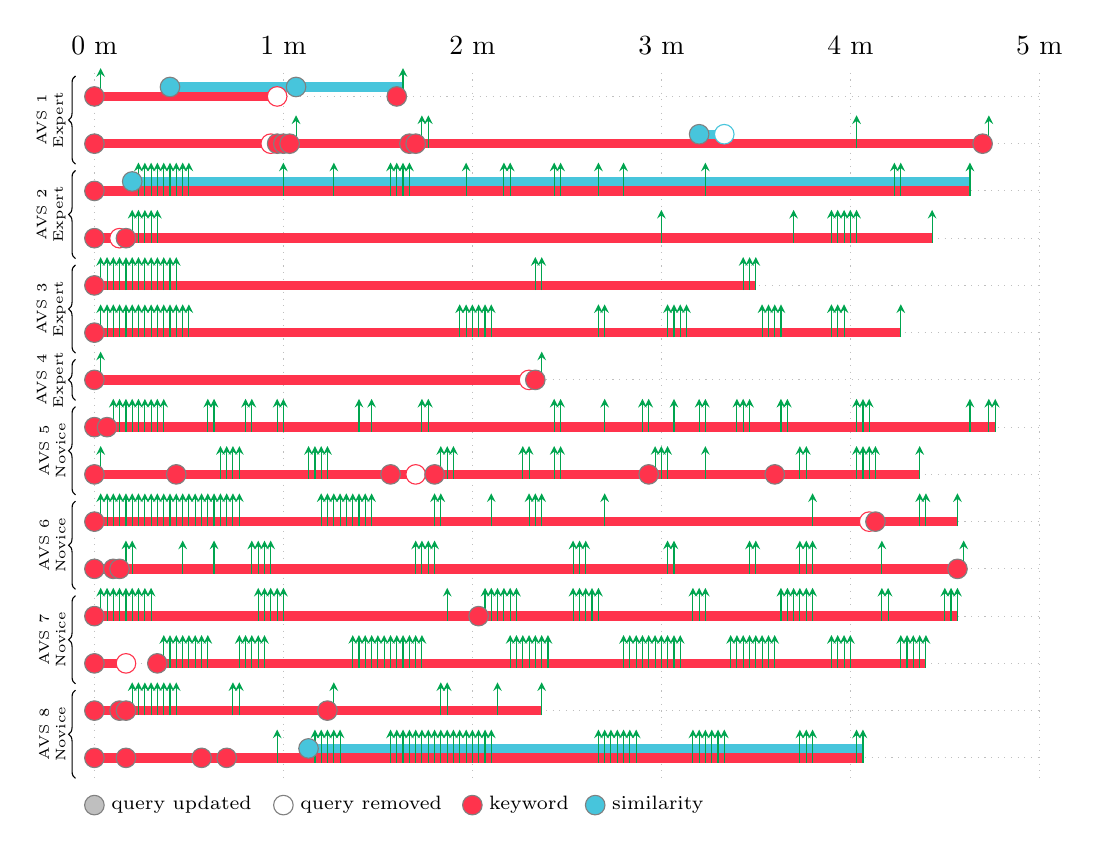
\begin{tikzpicture}[scale=2,x=1.2cm]
\usetikzlibrary{shapes}
\definecolor{YellowGreen}{RGB}{255,51,76}
\definecolor{SkyBlue}{RGB}{71,197,220}
\definecolor{Green}{RGB}{0,165,79}
\definecolor{Red}{RGB}{237,27,36}
\definecolor{Dandelion}{RGB}{253,189,66}
% draw horizontal line   
\draw[dotted,lightgray] (0,-0.150) -- (5,-0.150); 

\draw[dotted,lightgray] (0,-0.450) -- (5,-0.450); 

\draw[dotted,lightgray] (0,-0.750) -- (5,-0.750); 

\draw[dotted,lightgray] (0,-1.050) -- (5,-1.050); 

\draw[dotted,lightgray] (0,-1.350) -- (5,-1.350); 

\draw[dotted,lightgray] (0,-1.650) -- (5,-1.650); 

\draw[dotted,lightgray] (0,-1.950) -- (5,-1.950); 

\draw[dotted,lightgray] (0,-2.250) -- (5,-2.250); 

\draw[dotted,lightgray] (0,-2.550) -- (5,-2.550); 

\draw[dotted,lightgray] (0,-2.850) -- (5,-2.850); 

\draw[dotted,lightgray] (0,-3.150) -- (5,-3.150); 

\draw[dotted,lightgray] (0,-3.450) -- (5,-3.450); 

\draw[dotted,lightgray] (0,-3.750) -- (5,-3.750); 

\draw[dotted,lightgray] (0,-4.050) -- (5,-4.050); 

\draw[dotted,lightgray] (0,-4.350) -- (5,-4.350);

% draw vertical lines
\foreach \x in {0,1,2,3,4,5}
\draw[dotted,lightgray] (\x,0) -- (\x,-2.40-2.1);

% draw nodes
\draw (0,0) node[above=3pt] {0 m};
\draw (1,0) node[above=3pt] {1 m};
\draw (2,0) node[above=3pt] {2 m};
\draw (3,0) node[above=3pt] {3 m};
\draw (4,0) node[above=3pt] {4 m};
\draw (5,0) node[above=3pt] {5 m};

\draw[decorate,decoration={brace}] (-0.1,-0.58) -- (-0.1,-0.02) node[midway, anchor=center, sloped, above=0.05, font=\tiny, align=center] {AVS 1 \\ Expert};
\draw[decorate,decoration={brace}] (-0.1,-1.18) -- (-0.1,-0.62) node[midway, anchor=center, sloped, above=0.05, font=\tiny, align=center] {AVS 2 \\ Expert};
\draw[decorate,decoration={brace}] (-0.1,-1.78) -- (-0.1,-1.22) node[midway, anchor=center, sloped, above=0.05, font=\tiny, align=center] {AVS 3 \\ Expert};
\draw[decorate,decoration={brace}] (-0.1,-2.08) -- (-0.1,-1.82) node[midway, anchor=center, sloped, above=0.05, font=\tiny, align=center] {AVS 4 \\ Expert};

\draw[decorate,decoration={brace}] (-0.1,-2.68) -- (-0.1,-2.12) node[midway, anchor=center, sloped, above=0.1, font=\tiny, align=center] {AVS 5 \\ Novice};
\draw[decorate,decoration={brace}] (-0.1,-3.28) -- (-0.1,-2.72) node[midway, anchor=center, sloped, above=0.1, font=\tiny, align=center] {AVS 6 \\ Novice};
\draw[decorate,decoration={brace}] (-0.1,-3.88) -- (-0.1,-3.32) node[midway, anchor=center, sloped, above=0.1, font=\tiny, align=center] {AVS 7 \\ Novice};
\draw[decorate,decoration={brace}] (-0.1,-4.48) -- (-0.1,-3.92) node[midway, anchor=center, sloped, above=0.1, font=\tiny, align=center] {AVS 8 \\ Novice};

\node[draw=gray, circle, fill=lightgray, inner sep=2.5pt, align=center]at (0,-2.55-2.1) {};
\node[anchor=west, font=\scriptsize]at (0.0375,-2.55-2.1) {query updated};
\node[draw=gray, circle, fill=white, inner sep=2.5pt, align=center]at (1,-2.55-2.1) {};
\node[anchor=west, font=\scriptsize]at (1.0375,-2.55-2.1) {query removed};

\node[draw=gray, circle, fill=YellowGreen, inner sep=2.5pt, align=center]at (2,-2.55-2.1) {};
\node[anchor=west, font=\scriptsize]at (2.0375,-2.55-2.1) {keyword};
\node[draw=gray, circle, fill=SkyBlue, inner sep=2.5pt, align=center]at (2.65,-2.55-2.1) {};
\node[anchor=west, font=\scriptsize]at (2.6875,-2.55-2.1) {similarity};
%\node[draw=gray, circle, fill=Dandelion, inner sep=2.5pt, align=center]at (2.7,-2.55-2.1) {};
%\node[anchor=west, font=\scriptsize]at (2.73,-2.55-2.1) {color};


\draw[line width=0.12cm, YellowGreen](0.000,-0.150 -0) -- (0.967,-0.150 -0);
\draw[line width=0.12cm, SkyBlue](0.400,-0.150 +0.06) -- (1.633,-0.150 +0.06);
\draw[line width=0.12cm, YellowGreen](1.600,-0.150 -0) -- (1.633,-0.150 -0);
\draw[-stealth,Green] (0.033,-0.150 -0.03) -- (0.033,-0.150 + 0.18);
\draw[-stealth,Green] (1.633,-0.150 -0.03) -- (1.633,-0.150 + 0.18);
\node[draw=gray, circle, fill=YellowGreen, inner sep=2.5pt, align=center]at (0.000,-0.150 -0) {};
\node[draw=gray, circle, fill=SkyBlue, inner sep=2.5pt, align=center]at (0.400,-0.150 +0.06) {};
\node[draw=YellowGreen, circle, fill=white, inner sep=2.5pt, align=center]at (0.967,-0.150 -0) {};
\node[draw=gray, circle, fill=SkyBlue, inner sep=2.5pt, align=center]at (1.067,-0.150 +0.06) {};
\node[draw=gray, circle, fill=YellowGreen, inner sep=2.5pt, align=center]at (1.600,-0.150 -0) {};


\draw[line width=0.12cm, YellowGreen](0.000,-0.450 -0) -- (0.933,-0.450 -0);
\draw[line width=0.12cm, SkyBlue](3.200,-0.450 +0.06) -- (3.333,-0.450 +0.06);
\draw[line width=0.12cm, YellowGreen](0.967,-0.450 -0) -- (4.733,-0.450 -0);
\draw[-stealth,Green] (1.067,-0.450 -0.03) -- (1.067,-0.450 + 0.18);
\draw[-stealth,Green] (1.733,-0.450 -0.03) -- (1.733,-0.450 + 0.18);
\draw[-stealth,Green] (1.767,-0.450 -0.03) -- (1.767,-0.450 + 0.18);
\draw[-stealth,Green] (4.033,-0.450 -0.03) -- (4.033,-0.450 + 0.18);
\draw[-stealth,Green] (4.733,-0.450 -0.03) -- (4.733,-0.450 + 0.18);
\node[draw=gray, circle, fill=YellowGreen, inner sep=2.5pt, align=center]at (0.000,-0.450 -0) {};
\node[draw=YellowGreen, circle, fill=white, inner sep=2.5pt, align=center]at (0.933,-0.450 -0) {};
\node[draw=gray, circle, fill=YellowGreen, inner sep=2.5pt, align=center]at (0.967,-0.450 -0) {};
\node[draw=gray, circle, fill=YellowGreen, inner sep=2.5pt, align=center]at (1.000,-0.450 -0) {};
\node[draw=gray, circle, fill=YellowGreen, inner sep=2.5pt, align=center]at (1.033,-0.450 -0) {};
\node[draw=gray, circle, fill=YellowGreen, inner sep=2.5pt, align=center]at (1.667,-0.450 -0) {};
\node[draw=gray, circle, fill=YellowGreen, inner sep=2.5pt, align=center]at (1.700,-0.450 -0) {};
\node[draw=gray, circle, fill=SkyBlue, inner sep=2.5pt, align=center]at (3.200,-0.450 +0.06) {};
\node[draw=SkyBlue, circle, fill=white, inner sep=2.5pt, align=center]at (3.333,-0.450 +0.06) {};
\node[draw=gray, circle, fill=YellowGreen, inner sep=2.5pt, align=center]at (4.700,-0.450 -0) {};


\draw[line width=0.12cm, SkyBlue](0.200,-0.750 +0.06) -- (4.633,-0.750 +0.06);
\draw[line width=0.12cm, YellowGreen](0.000,-0.750 -0) -- (4.633,-0.750 -0);
\draw[-stealth,Green] (0.233,-0.750 -0.03) -- (0.233,-0.750 + 0.18);
\draw[-stealth,Green] (0.267,-0.750 -0.03) -- (0.267,-0.750 + 0.18);
\draw[-stealth,Green] (0.300,-0.750 -0.03) -- (0.300,-0.750 + 0.18);
\draw[-stealth,Green] (0.333,-0.750 -0.03) -- (0.333,-0.750 + 0.18);
\draw[-stealth,Green] (0.367,-0.750 -0.03) -- (0.367,-0.750 + 0.18);
\draw[-stealth,Green] (0.400,-0.750 -0.03) -- (0.400,-0.750 + 0.18);
\draw[-stealth,Green] (0.433,-0.750 -0.03) -- (0.433,-0.750 + 0.18);
\draw[-stealth,Green] (0.467,-0.750 -0.03) -- (0.467,-0.750 + 0.18);
\draw[-stealth,Green] (0.500,-0.750 -0.03) -- (0.500,-0.750 + 0.18);
\draw[-stealth,Green] (1.000,-0.750 -0.03) -- (1.000,-0.750 + 0.18);
\draw[-stealth,Green] (1.267,-0.750 -0.03) -- (1.267,-0.750 + 0.18);
\draw[-stealth,Green] (1.567,-0.750 -0.03) -- (1.567,-0.750 + 0.18);
\draw[-stealth,Green] (1.600,-0.750 -0.03) -- (1.600,-0.750 + 0.18);
\draw[-stealth,Green] (1.633,-0.750 -0.03) -- (1.633,-0.750 + 0.18);
\draw[-stealth,Green] (1.667,-0.750 -0.03) -- (1.667,-0.750 + 0.18);
\draw[-stealth,Green] (1.967,-0.750 -0.03) -- (1.967,-0.750 + 0.18);
\draw[-stealth,Green] (2.167,-0.750 -0.03) -- (2.167,-0.750 + 0.18);
\draw[-stealth,Green] (2.200,-0.750 -0.03) -- (2.200,-0.750 + 0.18);
\draw[-stealth,Green] (2.433,-0.750 -0.03) -- (2.433,-0.750 + 0.18);
\draw[-stealth,Green] (2.467,-0.750 -0.03) -- (2.467,-0.750 + 0.18);
\draw[-stealth,Green] (2.667,-0.750 -0.03) -- (2.667,-0.750 + 0.18);
\draw[-stealth,Green] (2.800,-0.750 -0.03) -- (2.800,-0.750 + 0.18);
\draw[-stealth,Green] (3.233,-0.750 -0.03) -- (3.233,-0.750 + 0.18);
\draw[-stealth,Green] (4.233,-0.750 -0.03) -- (4.233,-0.750 + 0.18);
\draw[-stealth,Green] (4.267,-0.750 -0.03) -- (4.267,-0.750 + 0.18);
\draw[-stealth,Green] (4.633,-0.750 -0.03) -- (4.633,-0.750 + 0.18);
\node[draw=gray, circle, fill=YellowGreen, inner sep=2.5pt, align=center]at (0.000,-0.750 -0) {};
\node[draw=gray, circle, fill=SkyBlue, inner sep=2.5pt, align=center]at (0.200,-0.750 +0.06) {};


\draw[line width=0.12cm, YellowGreen](0.000,-1.050 -0) -- (0.133,-1.050 -0);
\draw[line width=0.12cm, YellowGreen](0.167,-1.050 -0) -- (4.433,-1.050 -0);
\draw[-stealth,Green] (0.200,-1.050 -0.03) -- (0.200,-1.050 + 0.18);
\draw[-stealth,Green] (0.233,-1.050 -0.03) -- (0.233,-1.050 + 0.18);
\draw[-stealth,Green] (0.267,-1.050 -0.03) -- (0.267,-1.050 + 0.18);
\draw[-stealth,Green] (0.300,-1.050 -0.03) -- (0.300,-1.050 + 0.18);
\draw[-stealth,Green] (0.333,-1.050 -0.03) -- (0.333,-1.050 + 0.18);
\draw[-stealth,Green] (3.000,-1.050 -0.03) -- (3.000,-1.050 + 0.18);
\draw[-stealth,Green] (3.700,-1.050 -0.03) -- (3.700,-1.050 + 0.18);
\draw[-stealth,Green] (3.900,-1.050 -0.03) -- (3.900,-1.050 + 0.18);
\draw[-stealth,Green] (3.933,-1.050 -0.03) -- (3.933,-1.050 + 0.18);
\draw[-stealth,Green] (3.967,-1.050 -0.03) -- (3.967,-1.050 + 0.18);
\draw[-stealth,Green] (4.000,-1.050 -0.03) -- (4.000,-1.050 + 0.18);
\draw[-stealth,Green] (4.033,-1.050 -0.03) -- (4.033,-1.050 + 0.18);
\draw[-stealth,Green] (4.433,-1.050 -0.03) -- (4.433,-1.050 + 0.18);
\node[draw=gray, circle, fill=YellowGreen, inner sep=2.5pt, align=center]at (0.000,-1.050 -0) {};
\node[draw=YellowGreen, circle, fill=white, inner sep=2.5pt, align=center]at (0.133,-1.050 -0) {};
\node[draw=gray, circle, fill=YellowGreen, inner sep=2.5pt, align=center]at (0.167,-1.050 -0) {};


\draw[line width=0.12cm, YellowGreen](0.000,-1.350 -0) -- (3.500,-1.350 -0);
\draw[-stealth,Green] (0.033,-1.350 -0.03) -- (0.033,-1.350 + 0.18);
\draw[-stealth,Green] (0.067,-1.350 -0.03) -- (0.067,-1.350 + 0.18);
\draw[-stealth,Green] (0.100,-1.350 -0.03) -- (0.100,-1.350 + 0.18);
\draw[-stealth,Green] (0.133,-1.350 -0.03) -- (0.133,-1.350 + 0.18);
\draw[-stealth,Green] (0.167,-1.350 -0.03) -- (0.167,-1.350 + 0.18);
\draw[-stealth,Green] (0.200,-1.350 -0.03) -- (0.200,-1.350 + 0.18);
\draw[-stealth,Green] (0.233,-1.350 -0.03) -- (0.233,-1.350 + 0.18);
\draw[-stealth,Green] (0.267,-1.350 -0.03) -- (0.267,-1.350 + 0.18);
\draw[-stealth,Green] (0.300,-1.350 -0.03) -- (0.300,-1.350 + 0.18);
\draw[-stealth,Green] (0.333,-1.350 -0.03) -- (0.333,-1.350 + 0.18);
\draw[-stealth,Green] (0.367,-1.350 -0.03) -- (0.367,-1.350 + 0.18);
\draw[-stealth,Green] (0.400,-1.350 -0.03) -- (0.400,-1.350 + 0.18);
\draw[-stealth,Green] (0.433,-1.350 -0.03) -- (0.433,-1.350 + 0.18);
\draw[-stealth,Green] (2.333,-1.350 -0.03) -- (2.333,-1.350 + 0.18);
\draw[-stealth,Green] (2.367,-1.350 -0.03) -- (2.367,-1.350 + 0.18);
\draw[-stealth,Green] (3.433,-1.350 -0.03) -- (3.433,-1.350 + 0.18);
\draw[-stealth,Green] (3.467,-1.350 -0.03) -- (3.467,-1.350 + 0.18);
\draw[-stealth,Green] (3.500,-1.350 -0.03) -- (3.500,-1.350 + 0.18);
\node[draw=gray, circle, fill=YellowGreen, inner sep=2.5pt, align=center]at (0.000,-1.350 -0) {};


\draw[line width=0.12cm, YellowGreen](0.000,-1.650 -0) -- (4.267,-1.650 -0);
\draw[-stealth,Green] (0.033,-1.650 -0.03) -- (0.033,-1.650 + 0.18);
\draw[-stealth,Green] (0.067,-1.650 -0.03) -- (0.067,-1.650 + 0.18);
\draw[-stealth,Green] (0.100,-1.650 -0.03) -- (0.100,-1.650 + 0.18);
\draw[-stealth,Green] (0.133,-1.650 -0.03) -- (0.133,-1.650 + 0.18);
\draw[-stealth,Green] (0.167,-1.650 -0.03) -- (0.167,-1.650 + 0.18);
\draw[-stealth,Green] (0.200,-1.650 -0.03) -- (0.200,-1.650 + 0.18);
\draw[-stealth,Green] (0.233,-1.650 -0.03) -- (0.233,-1.650 + 0.18);
\draw[-stealth,Green] (0.267,-1.650 -0.03) -- (0.267,-1.650 + 0.18);
\draw[-stealth,Green] (0.300,-1.650 -0.03) -- (0.300,-1.650 + 0.18);
\draw[-stealth,Green] (0.333,-1.650 -0.03) -- (0.333,-1.650 + 0.18);
\draw[-stealth,Green] (0.367,-1.650 -0.03) -- (0.367,-1.650 + 0.18);
\draw[-stealth,Green] (0.400,-1.650 -0.03) -- (0.400,-1.650 + 0.18);
\draw[-stealth,Green] (0.433,-1.650 -0.03) -- (0.433,-1.650 + 0.18);
\draw[-stealth,Green] (0.467,-1.650 -0.03) -- (0.467,-1.650 + 0.18);
\draw[-stealth,Green] (0.500,-1.650 -0.03) -- (0.500,-1.650 + 0.18);
\draw[-stealth,Green] (1.933,-1.650 -0.03) -- (1.933,-1.650 + 0.18);
\draw[-stealth,Green] (1.967,-1.650 -0.03) -- (1.967,-1.650 + 0.18);
\draw[-stealth,Green] (2.000,-1.650 -0.03) -- (2.000,-1.650 + 0.18);
\draw[-stealth,Green] (2.033,-1.650 -0.03) -- (2.033,-1.650 + 0.18);
\draw[-stealth,Green] (2.067,-1.650 -0.03) -- (2.067,-1.650 + 0.18);
\draw[-stealth,Green] (2.100,-1.650 -0.03) -- (2.100,-1.650 + 0.18);
\draw[-stealth,Green] (2.667,-1.650 -0.03) -- (2.667,-1.650 + 0.18);
\draw[-stealth,Green] (2.700,-1.650 -0.03) -- (2.700,-1.650 + 0.18);
\draw[-stealth,Green] (3.033,-1.650 -0.03) -- (3.033,-1.650 + 0.18);
\draw[-stealth,Green] (3.067,-1.650 -0.03) -- (3.067,-1.650 + 0.18);
\draw[-stealth,Green] (3.100,-1.650 -0.03) -- (3.100,-1.650 + 0.18);
\draw[-stealth,Green] (3.133,-1.650 -0.03) -- (3.133,-1.650 + 0.18);
\draw[-stealth,Green] (3.533,-1.650 -0.03) -- (3.533,-1.650 + 0.18);
\draw[-stealth,Green] (3.567,-1.650 -0.03) -- (3.567,-1.650 + 0.18);
\draw[-stealth,Green] (3.600,-1.650 -0.03) -- (3.600,-1.650 + 0.18);
\draw[-stealth,Green] (3.633,-1.650 -0.03) -- (3.633,-1.650 + 0.18);
\draw[-stealth,Green] (3.900,-1.650 -0.03) -- (3.900,-1.650 + 0.18);
\draw[-stealth,Green] (3.933,-1.650 -0.03) -- (3.933,-1.650 + 0.18);
\draw[-stealth,Green] (3.967,-1.650 -0.03) -- (3.967,-1.650 + 0.18);
\draw[-stealth,Green] (4.267,-1.650 -0.03) -- (4.267,-1.650 + 0.18);
\node[draw=gray, circle, fill=YellowGreen, inner sep=2.5pt, align=center]at (0.000,-1.650 -0) {};


\draw[line width=0.12cm, YellowGreen](0.000,-1.950 -0) -- (2.300,-1.950 -0);
\draw[line width=0.12cm, YellowGreen](2.333,-1.950 -0) -- (2.367,-1.950 -0);
\draw[-stealth,Green] (0.033,-1.950 -0.03) -- (0.033,-1.950 + 0.18);
\draw[-stealth,Green] (2.367,-1.950 -0.03) -- (2.367,-1.950 + 0.18);
\node[draw=gray, circle, fill=YellowGreen, inner sep=2.5pt, align=center]at (0.000,-1.950 -0) {};
\node[draw=YellowGreen, circle, fill=white, inner sep=2.5pt, align=center]at (2.300,-1.950 -0) {};
\node[draw=gray, circle, fill=YellowGreen, inner sep=2.5pt, align=center]at (2.333,-1.950 -0) {};

% novice
\draw[line width=0.12cm, YellowGreen](0.000,-2.250 -0) -- (4.767,-2.250 -0);
\draw[-stealth,Green] (0.100,-2.250 -0.03) -- (0.100,-2.250 + 0.18);
\draw[-stealth,Green] (0.133,-2.250 -0.03) -- (0.133,-2.250 + 0.18);
\draw[-stealth,Green] (0.167,-2.250 -0.03) -- (0.167,-2.250 + 0.18);
\draw[-stealth,Green] (0.200,-2.250 -0.03) -- (0.200,-2.250 + 0.18);
\draw[-stealth,Green] (0.233,-2.250 -0.03) -- (0.233,-2.250 + 0.18);
\draw[-stealth,Green] (0.267,-2.250 -0.03) -- (0.267,-2.250 + 0.18);
\draw[-stealth,Green] (0.300,-2.250 -0.03) -- (0.300,-2.250 + 0.18);
\draw[-stealth,Green] (0.333,-2.250 -0.03) -- (0.333,-2.250 + 0.18);
\draw[-stealth,Green] (0.367,-2.250 -0.03) -- (0.367,-2.250 + 0.18);
\draw[-stealth,Green] (0.600,-2.250 -0.03) -- (0.600,-2.250 + 0.18);
\draw[-stealth,Green] (0.633,-2.250 -0.03) -- (0.633,-2.250 + 0.18);
\draw[-stealth,Green] (0.800,-2.250 -0.03) -- (0.800,-2.250 + 0.18);
\draw[-stealth,Green] (0.833,-2.250 -0.03) -- (0.833,-2.250 + 0.18);
\draw[-stealth,Green] (0.967,-2.250 -0.03) -- (0.967,-2.250 + 0.18);
\draw[-stealth,Green] (1.000,-2.250 -0.03) -- (1.000,-2.250 + 0.18);
\draw[-stealth,Green] (1.400,-2.250 -0.03) -- (1.400,-2.250 + 0.18);
\draw[-stealth,Green] (1.467,-2.250 -0.03) -- (1.467,-2.250 + 0.18);
\draw[-stealth,Green] (1.733,-2.250 -0.03) -- (1.733,-2.250 + 0.18);
\draw[-stealth,Green] (1.767,-2.250 -0.03) -- (1.767,-2.250 + 0.18);
\draw[-stealth,Green] (2.433,-2.250 -0.03) -- (2.433,-2.250 + 0.18);
\draw[-stealth,Green] (2.467,-2.250 -0.03) -- (2.467,-2.250 + 0.18);
\draw[-stealth,Green] (2.700,-2.250 -0.03) -- (2.700,-2.250 + 0.18);
\draw[-stealth,Green] (2.900,-2.250 -0.03) -- (2.900,-2.250 + 0.18);
\draw[-stealth,Green] (2.933,-2.250 -0.03) -- (2.933,-2.250 + 0.18);
\draw[-stealth,Green] (3.067,-2.250 -0.03) -- (3.067,-2.250 + 0.18);
\draw[-stealth,Green] (3.200,-2.250 -0.03) -- (3.200,-2.250 + 0.18);
\draw[-stealth,Green] (3.233,-2.250 -0.03) -- (3.233,-2.250 + 0.18);
\draw[-stealth,Green] (3.400,-2.250 -0.03) -- (3.400,-2.250 + 0.18);
\draw[-stealth,Green] (3.433,-2.250 -0.03) -- (3.433,-2.250 + 0.18);
\draw[-stealth,Green] (3.467,-2.250 -0.03) -- (3.467,-2.250 + 0.18);
\draw[-stealth,Green] (3.633,-2.250 -0.03) -- (3.633,-2.250 + 0.18);
\draw[-stealth,Green] (3.667,-2.250 -0.03) -- (3.667,-2.250 + 0.18);
\draw[-stealth,Green] (4.033,-2.250 -0.03) -- (4.033,-2.250 + 0.18);
\draw[-stealth,Green] (4.067,-2.250 -0.03) -- (4.067,-2.250 + 0.18);
\draw[-stealth,Green] (4.100,-2.250 -0.03) -- (4.100,-2.250 + 0.18);
\draw[-stealth,Green] (4.633,-2.250 -0.03) -- (4.633,-2.250 + 0.18);
\draw[-stealth,Green] (4.733,-2.250 -0.03) -- (4.733,-2.250 + 0.18);
\draw[-stealth,Green] (4.767,-2.250 -0.03) -- (4.767,-2.250 + 0.18);
\node[draw=gray, circle, fill=YellowGreen, inner sep=2.5pt, align=center]at (0.000,-2.250 -0) {};
\node[draw=gray, circle, fill=YellowGreen, inner sep=2.5pt, align=center]at (0.067,-2.250 -0) {};


\draw[line width=0.12cm, YellowGreen](0.000,-2.550 -0) -- (1.700,-2.550 -0);
\draw[line width=0.12cm, YellowGreen](1.800,-2.550 -0) -- (4.367,-2.550 -0);
\draw[-stealth,Green] (0.033,-2.550 -0.03) -- (0.033,-2.550 + 0.18);
\draw[-stealth,Green] (0.667,-2.550 -0.03) -- (0.667,-2.550 + 0.18);
\draw[-stealth,Green] (0.700,-2.550 -0.03) -- (0.700,-2.550 + 0.18);
\draw[-stealth,Green] (0.733,-2.550 -0.03) -- (0.733,-2.550 + 0.18);
\draw[-stealth,Green] (0.767,-2.550 -0.03) -- (0.767,-2.550 + 0.18);
\draw[-stealth,Green] (1.133,-2.550 -0.03) -- (1.133,-2.550 + 0.18);
\draw[-stealth,Green] (1.167,-2.550 -0.03) -- (1.167,-2.550 + 0.18);
\draw[-stealth,Green] (1.200,-2.550 -0.03) -- (1.200,-2.550 + 0.18);
\draw[-stealth,Green] (1.233,-2.550 -0.03) -- (1.233,-2.550 + 0.18);
\draw[-stealth,Green] (1.833,-2.550 -0.03) -- (1.833,-2.550 + 0.18);
\draw[-stealth,Green] (1.867,-2.550 -0.03) -- (1.867,-2.550 + 0.18);
\draw[-stealth,Green] (1.900,-2.550 -0.03) -- (1.900,-2.550 + 0.18);
\draw[-stealth,Green] (2.267,-2.550 -0.03) -- (2.267,-2.550 + 0.18);
\draw[-stealth,Green] (2.300,-2.550 -0.03) -- (2.300,-2.550 + 0.18);
\draw[-stealth,Green] (2.433,-2.550 -0.03) -- (2.433,-2.550 + 0.18);
\draw[-stealth,Green] (2.467,-2.550 -0.03) -- (2.467,-2.550 + 0.18);
\draw[-stealth,Green] (2.967,-2.550 -0.03) -- (2.967,-2.550 + 0.18);
\draw[-stealth,Green] (3.000,-2.550 -0.03) -- (3.000,-2.550 + 0.18);
\draw[-stealth,Green] (3.033,-2.550 -0.03) -- (3.033,-2.550 + 0.18);
\draw[-stealth,Green] (3.233,-2.550 -0.03) -- (3.233,-2.550 + 0.18);
\draw[-stealth,Green] (3.733,-2.550 -0.03) -- (3.733,-2.550 + 0.18);
\draw[-stealth,Green] (3.767,-2.550 -0.03) -- (3.767,-2.550 + 0.18);
\draw[-stealth,Green] (4.033,-2.550 -0.03) -- (4.033,-2.550 + 0.18);
\draw[-stealth,Green] (4.067,-2.550 -0.03) -- (4.067,-2.550 + 0.18);
\draw[-stealth,Green] (4.100,-2.550 -0.03) -- (4.100,-2.550 + 0.18);
\draw[-stealth,Green] (4.133,-2.550 -0.03) -- (4.133,-2.550 + 0.18);
\draw[-stealth,Green] (4.367,-2.550 -0.03) -- (4.367,-2.550 + 0.18);
\node[draw=gray, circle, fill=YellowGreen, inner sep=2.5pt, align=center]at (0.000,-2.550 -0) {};
\node[draw=gray, circle, fill=YellowGreen, inner sep=2.5pt, align=center]at (0.433,-2.550 -0) {};
\node[draw=gray, circle, fill=YellowGreen, inner sep=2.5pt, align=center]at (1.567,-2.550 -0) {};
\node[draw=YellowGreen, circle, fill=white, inner sep=2.5pt, align=center]at (1.700,-2.550 -0) {};
\node[draw=gray, circle, fill=YellowGreen, inner sep=2.5pt, align=center]at (1.800,-2.550 -0) {};
\node[draw=gray, circle, fill=YellowGreen, inner sep=2.5pt, align=center]at (2.933,-2.550 -0) {};
\node[draw=gray, circle, fill=YellowGreen, inner sep=2.5pt, align=center]at (3.600,-2.550 -0) {};


\draw[line width=0.12cm, YellowGreen](0.000,-2.850 -0) -- (4.100,-2.850 -0);
\draw[line width=0.12cm, YellowGreen](4.133,-2.850 -0) -- (4.567,-2.850 -0);
\draw[-stealth,Green] (0.033,-2.850 -0.03) -- (0.033,-2.850 + 0.18);
\draw[-stealth,Green] (0.067,-2.850 -0.03) -- (0.067,-2.850 + 0.18);
\draw[-stealth,Green] (0.100,-2.850 -0.03) -- (0.100,-2.850 + 0.18);
\draw[-stealth,Green] (0.133,-2.850 -0.03) -- (0.133,-2.850 + 0.18);
\draw[-stealth,Green] (0.167,-2.850 -0.03) -- (0.167,-2.850 + 0.18);
\draw[-stealth,Green] (0.200,-2.850 -0.03) -- (0.200,-2.850 + 0.18);
\draw[-stealth,Green] (0.233,-2.850 -0.03) -- (0.233,-2.850 + 0.18);
\draw[-stealth,Green] (0.267,-2.850 -0.03) -- (0.267,-2.850 + 0.18);
\draw[-stealth,Green] (0.300,-2.850 -0.03) -- (0.300,-2.850 + 0.18);
\draw[-stealth,Green] (0.333,-2.850 -0.03) -- (0.333,-2.850 + 0.18);
\draw[-stealth,Green] (0.367,-2.850 -0.03) -- (0.367,-2.850 + 0.18);
\draw[-stealth,Green] (0.400,-2.850 -0.03) -- (0.400,-2.850 + 0.18);
\draw[-stealth,Green] (0.433,-2.850 -0.03) -- (0.433,-2.850 + 0.18);
\draw[-stealth,Green] (0.467,-2.850 -0.03) -- (0.467,-2.850 + 0.18);
\draw[-stealth,Green] (0.500,-2.850 -0.03) -- (0.500,-2.850 + 0.18);
\draw[-stealth,Green] (0.533,-2.850 -0.03) -- (0.533,-2.850 + 0.18);
\draw[-stealth,Green] (0.567,-2.850 -0.03) -- (0.567,-2.850 + 0.18);
\draw[-stealth,Green] (0.600,-2.850 -0.03) -- (0.600,-2.850 + 0.18);
\draw[-stealth,Green] (0.633,-2.850 -0.03) -- (0.633,-2.850 + 0.18);
\draw[-stealth,Green] (0.667,-2.850 -0.03) -- (0.667,-2.850 + 0.18);
\draw[-stealth,Green] (0.700,-2.850 -0.03) -- (0.700,-2.850 + 0.18);
\draw[-stealth,Green] (0.733,-2.850 -0.03) -- (0.733,-2.850 + 0.18);
\draw[-stealth,Green] (0.767,-2.850 -0.03) -- (0.767,-2.850 + 0.18);
\draw[-stealth,Green] (1.200,-2.850 -0.03) -- (1.200,-2.850 + 0.18);
\draw[-stealth,Green] (1.233,-2.850 -0.03) -- (1.233,-2.850 + 0.18);
\draw[-stealth,Green] (1.267,-2.850 -0.03) -- (1.267,-2.850 + 0.18);
\draw[-stealth,Green] (1.300,-2.850 -0.03) -- (1.300,-2.850 + 0.18);
\draw[-stealth,Green] (1.333,-2.850 -0.03) -- (1.333,-2.850 + 0.18);
\draw[-stealth,Green] (1.367,-2.850 -0.03) -- (1.367,-2.850 + 0.18);
\draw[-stealth,Green] (1.400,-2.850 -0.03) -- (1.400,-2.850 + 0.18);
\draw[-stealth,Green] (1.433,-2.850 -0.03) -- (1.433,-2.850 + 0.18);
\draw[-stealth,Green] (1.467,-2.850 -0.03) -- (1.467,-2.850 + 0.18);
\draw[-stealth,Green] (1.800,-2.850 -0.03) -- (1.800,-2.850 + 0.18);
\draw[-stealth,Green] (1.833,-2.850 -0.03) -- (1.833,-2.850 + 0.18);
\draw[-stealth,Green] (2.100,-2.850 -0.03) -- (2.100,-2.850 + 0.18);
\draw[-stealth,Green] (2.300,-2.850 -0.03) -- (2.300,-2.850 + 0.18);
\draw[-stealth,Green] (2.333,-2.850 -0.03) -- (2.333,-2.850 + 0.18);
\draw[-stealth,Green] (2.367,-2.850 -0.03) -- (2.367,-2.850 + 0.18);
\draw[-stealth,Green] (2.700,-2.850 -0.03) -- (2.700,-2.850 + 0.18);
\draw[-stealth,Green] (3.800,-2.850 -0.03) -- (3.800,-2.850 + 0.18);
\draw[-stealth,Green] (4.367,-2.850 -0.03) -- (4.367,-2.850 + 0.18);
\draw[-stealth,Green] (4.400,-2.850 -0.03) -- (4.400,-2.850 + 0.18);
\draw[-stealth,Green] (4.567,-2.850 -0.03) -- (4.567,-2.850 + 0.18);
\node[draw=gray, circle, fill=YellowGreen, inner sep=2.5pt, align=center]at (0.000,-2.850 -0) {};
\node[draw=YellowGreen, circle, fill=white, inner sep=2.5pt, align=center]at (4.100,-2.850 -0) {};
\node[draw=gray, circle, fill=YellowGreen, inner sep=2.5pt, align=center]at (4.133,-2.850 -0) {};


\draw[line width=0.12cm, YellowGreen](0.000,-3.150 -0) -- (4.600,-3.150 -0);
\draw[-stealth,Green] (0.167,-3.150 -0.03) -- (0.167,-3.150 + 0.18);
\draw[-stealth,Green] (0.200,-3.150 -0.03) -- (0.200,-3.150 + 0.18);
\draw[-stealth,Green] (0.467,-3.150 -0.03) -- (0.467,-3.150 + 0.18);
\draw[-stealth,Green] (0.633,-3.150 -0.03) -- (0.633,-3.150 + 0.18);
\draw[-stealth,Green] (0.833,-3.150 -0.03) -- (0.833,-3.150 + 0.18);
\draw[-stealth,Green] (0.867,-3.150 -0.03) -- (0.867,-3.150 + 0.18);
\draw[-stealth,Green] (0.900,-3.150 -0.03) -- (0.900,-3.150 + 0.18);
\draw[-stealth,Green] (0.933,-3.150 -0.03) -- (0.933,-3.150 + 0.18);
\draw[-stealth,Green] (1.700,-3.150 -0.03) -- (1.700,-3.150 + 0.18);
\draw[-stealth,Green] (1.733,-3.150 -0.03) -- (1.733,-3.150 + 0.18);
\draw[-stealth,Green] (1.767,-3.150 -0.03) -- (1.767,-3.150 + 0.18);
\draw[-stealth,Green] (1.800,-3.150 -0.03) -- (1.800,-3.150 + 0.18);
\draw[-stealth,Green] (2.533,-3.150 -0.03) -- (2.533,-3.150 + 0.18);
\draw[-stealth,Green] (2.567,-3.150 -0.03) -- (2.567,-3.150 + 0.18);
\draw[-stealth,Green] (2.600,-3.150 -0.03) -- (2.600,-3.150 + 0.18);
\draw[-stealth,Green] (3.033,-3.150 -0.03) -- (3.033,-3.150 + 0.18);
\draw[-stealth,Green] (3.067,-3.150 -0.03) -- (3.067,-3.150 + 0.18);
\draw[-stealth,Green] (3.467,-3.150 -0.03) -- (3.467,-3.150 + 0.18);
\draw[-stealth,Green] (3.500,-3.150 -0.03) -- (3.500,-3.150 + 0.18);
\draw[-stealth,Green] (3.733,-3.150 -0.03) -- (3.733,-3.150 + 0.18);
\draw[-stealth,Green] (3.767,-3.150 -0.03) -- (3.767,-3.150 + 0.18);
\draw[-stealth,Green] (3.800,-3.150 -0.03) -- (3.800,-3.150 + 0.18);
\draw[-stealth,Green] (4.167,-3.150 -0.03) -- (4.167,-3.150 + 0.18);
\draw[-stealth,Green] (4.600,-3.150 -0.03) -- (4.600,-3.150 + 0.18);
\node[draw=gray, circle, fill=YellowGreen, inner sep=2.5pt, align=center]at (0.000,-3.150 -0) {};
\node[draw=gray, circle, fill=YellowGreen, inner sep=2.5pt, align=center]at (0.100,-3.150 -0) {};
\node[draw=gray, circle, fill=YellowGreen, inner sep=2.5pt, align=center]at (0.133,-3.150 -0) {};
\node[draw=gray, circle, fill=YellowGreen, inner sep=2.5pt, align=center]at (4.567,-3.150 -0) {};


\draw[line width=0.12cm, YellowGreen](0.000,-3.450 -0) -- (4.567,-3.450 -0);
\draw[-stealth,Green] (0.033,-3.450 -0.03) -- (0.033,-3.450 + 0.18);
\draw[-stealth,Green] (0.067,-3.450 -0.03) -- (0.067,-3.450 + 0.18);
\draw[-stealth,Green] (0.100,-3.450 -0.03) -- (0.100,-3.450 + 0.18);
\draw[-stealth,Green] (0.133,-3.450 -0.03) -- (0.133,-3.450 + 0.18);
\draw[-stealth,Green] (0.167,-3.450 -0.03) -- (0.167,-3.450 + 0.18);
\draw[-stealth,Green] (0.200,-3.450 -0.03) -- (0.200,-3.450 + 0.18);
\draw[-stealth,Green] (0.233,-3.450 -0.03) -- (0.233,-3.450 + 0.18);
\draw[-stealth,Green] (0.267,-3.450 -0.03) -- (0.267,-3.450 + 0.18);
\draw[-stealth,Green] (0.300,-3.450 -0.03) -- (0.300,-3.450 + 0.18);
\draw[-stealth,Green] (0.867,-3.450 -0.03) -- (0.867,-3.450 + 0.18);
\draw[-stealth,Green] (0.900,-3.450 -0.03) -- (0.900,-3.450 + 0.18);
\draw[-stealth,Green] (0.933,-3.450 -0.03) -- (0.933,-3.450 + 0.18);
\draw[-stealth,Green] (0.967,-3.450 -0.03) -- (0.967,-3.450 + 0.18);
\draw[-stealth,Green] (1.000,-3.450 -0.03) -- (1.000,-3.450 + 0.18);
\draw[-stealth,Green] (1.867,-3.450 -0.03) -- (1.867,-3.450 + 0.18);
\draw[-stealth,Green] (2.067,-3.450 -0.03) -- (2.067,-3.450 + 0.18);
\draw[-stealth,Green] (2.100,-3.450 -0.03) -- (2.100,-3.450 + 0.18);
\draw[-stealth,Green] (2.133,-3.450 -0.03) -- (2.133,-3.450 + 0.18);
\draw[-stealth,Green] (2.167,-3.450 -0.03) -- (2.167,-3.450 + 0.18);
\draw[-stealth,Green] (2.200,-3.450 -0.03) -- (2.200,-3.450 + 0.18);
\draw[-stealth,Green] (2.233,-3.450 -0.03) -- (2.233,-3.450 + 0.18);
\draw[-stealth,Green] (2.533,-3.450 -0.03) -- (2.533,-3.450 + 0.18);
\draw[-stealth,Green] (2.567,-3.450 -0.03) -- (2.567,-3.450 + 0.18);
\draw[-stealth,Green] (2.600,-3.450 -0.03) -- (2.600,-3.450 + 0.18);
\draw[-stealth,Green] (2.633,-3.450 -0.03) -- (2.633,-3.450 + 0.18);
\draw[-stealth,Green] (2.667,-3.450 -0.03) -- (2.667,-3.450 + 0.18);
\draw[-stealth,Green] (3.167,-3.450 -0.03) -- (3.167,-3.450 + 0.18);
\draw[-stealth,Green] (3.200,-3.450 -0.03) -- (3.200,-3.450 + 0.18);
\draw[-stealth,Green] (3.233,-3.450 -0.03) -- (3.233,-3.450 + 0.18);
\draw[-stealth,Green] (3.633,-3.450 -0.03) -- (3.633,-3.450 + 0.18);
\draw[-stealth,Green] (3.667,-3.450 -0.03) -- (3.667,-3.450 + 0.18);
\draw[-stealth,Green] (3.700,-3.450 -0.03) -- (3.700,-3.450 + 0.18);
\draw[-stealth,Green] (3.733,-3.450 -0.03) -- (3.733,-3.450 + 0.18);
\draw[-stealth,Green] (3.767,-3.450 -0.03) -- (3.767,-3.450 + 0.18);
\draw[-stealth,Green] (3.800,-3.450 -0.03) -- (3.800,-3.450 + 0.18);
\draw[-stealth,Green] (4.167,-3.450 -0.03) -- (4.167,-3.450 + 0.18);
\draw[-stealth,Green] (4.200,-3.450 -0.03) -- (4.200,-3.450 + 0.18);
\draw[-stealth,Green] (4.500,-3.450 -0.03) -- (4.500,-3.450 + 0.18);
\draw[-stealth,Green] (4.533,-3.450 -0.03) -- (4.533,-3.450 + 0.18);
\draw[-stealth,Green] (4.567,-3.450 -0.03) -- (4.567,-3.450 + 0.18);
\node[draw=gray, circle, fill=YellowGreen, inner sep=2.5pt, align=center]at (0.000,-3.450 -0) {};
\node[draw=gray, circle, fill=YellowGreen, inner sep=2.5pt, align=center]at (2.033,-3.450 -0) {};


\draw[line width=0.12cm, YellowGreen](0.000,-3.750 -0) -- (0.167,-3.750 -0);
\draw[line width=0.12cm, YellowGreen](0.333,-3.750 -0) -- (4.400,-3.750 -0);
\draw[-stealth,Green] (0.367,-3.750 -0.03) -- (0.367,-3.750 + 0.18);
\draw[-stealth,Green] (0.400,-3.750 -0.03) -- (0.400,-3.750 + 0.18);
\draw[-stealth,Green] (0.433,-3.750 -0.03) -- (0.433,-3.750 + 0.18);
\draw[-stealth,Green] (0.467,-3.750 -0.03) -- (0.467,-3.750 + 0.18);
\draw[-stealth,Green] (0.500,-3.750 -0.03) -- (0.500,-3.750 + 0.18);
\draw[-stealth,Green] (0.533,-3.750 -0.03) -- (0.533,-3.750 + 0.18);
\draw[-stealth,Green] (0.567,-3.750 -0.03) -- (0.567,-3.750 + 0.18);
\draw[-stealth,Green] (0.600,-3.750 -0.03) -- (0.600,-3.750 + 0.18);
\draw[-stealth,Green] (0.767,-3.750 -0.03) -- (0.767,-3.750 + 0.18);
\draw[-stealth,Green] (0.800,-3.750 -0.03) -- (0.800,-3.750 + 0.18);
\draw[-stealth,Green] (0.833,-3.750 -0.03) -- (0.833,-3.750 + 0.18);
\draw[-stealth,Green] (0.867,-3.750 -0.03) -- (0.867,-3.750 + 0.18);
\draw[-stealth,Green] (0.900,-3.750 -0.03) -- (0.900,-3.750 + 0.18);
\draw[-stealth,Green] (1.367,-3.750 -0.03) -- (1.367,-3.750 + 0.18);
\draw[-stealth,Green] (1.400,-3.750 -0.03) -- (1.400,-3.750 + 0.18);
\draw[-stealth,Green] (1.433,-3.750 -0.03) -- (1.433,-3.750 + 0.18);
\draw[-stealth,Green] (1.467,-3.750 -0.03) -- (1.467,-3.750 + 0.18);
\draw[-stealth,Green] (1.500,-3.750 -0.03) -- (1.500,-3.750 + 0.18);
\draw[-stealth,Green] (1.533,-3.750 -0.03) -- (1.533,-3.750 + 0.18);
\draw[-stealth,Green] (1.567,-3.750 -0.03) -- (1.567,-3.750 + 0.18);
\draw[-stealth,Green] (1.600,-3.750 -0.03) -- (1.600,-3.750 + 0.18);
\draw[-stealth,Green] (1.633,-3.750 -0.03) -- (1.633,-3.750 + 0.18);
\draw[-stealth,Green] (1.667,-3.750 -0.03) -- (1.667,-3.750 + 0.18);
\draw[-stealth,Green] (1.700,-3.750 -0.03) -- (1.700,-3.750 + 0.18);
\draw[-stealth,Green] (1.733,-3.750 -0.03) -- (1.733,-3.750 + 0.18);
\draw[-stealth,Green] (2.200,-3.750 -0.03) -- (2.200,-3.750 + 0.18);
\draw[-stealth,Green] (2.233,-3.750 -0.03) -- (2.233,-3.750 + 0.18);
\draw[-stealth,Green] (2.267,-3.750 -0.03) -- (2.267,-3.750 + 0.18);
\draw[-stealth,Green] (2.300,-3.750 -0.03) -- (2.300,-3.750 + 0.18);
\draw[-stealth,Green] (2.333,-3.750 -0.03) -- (2.333,-3.750 + 0.18);
\draw[-stealth,Green] (2.367,-3.750 -0.03) -- (2.367,-3.750 + 0.18);
\draw[-stealth,Green] (2.400,-3.750 -0.03) -- (2.400,-3.750 + 0.18);
\draw[-stealth,Green] (2.800,-3.750 -0.03) -- (2.800,-3.750 + 0.18);
\draw[-stealth,Green] (2.833,-3.750 -0.03) -- (2.833,-3.750 + 0.18);
\draw[-stealth,Green] (2.867,-3.750 -0.03) -- (2.867,-3.750 + 0.18);
\draw[-stealth,Green] (2.900,-3.750 -0.03) -- (2.900,-3.750 + 0.18);
\draw[-stealth,Green] (2.933,-3.750 -0.03) -- (2.933,-3.750 + 0.18);
\draw[-stealth,Green] (2.967,-3.750 -0.03) -- (2.967,-3.750 + 0.18);
\draw[-stealth,Green] (3.000,-3.750 -0.03) -- (3.000,-3.750 + 0.18);
\draw[-stealth,Green] (3.033,-3.750 -0.03) -- (3.033,-3.750 + 0.18);
\draw[-stealth,Green] (3.067,-3.750 -0.03) -- (3.067,-3.750 + 0.18);
\draw[-stealth,Green] (3.100,-3.750 -0.03) -- (3.100,-3.750 + 0.18);
\draw[-stealth,Green] (3.367,-3.750 -0.03) -- (3.367,-3.750 + 0.18);
\draw[-stealth,Green] (3.400,-3.750 -0.03) -- (3.400,-3.750 + 0.18);
\draw[-stealth,Green] (3.433,-3.750 -0.03) -- (3.433,-3.750 + 0.18);
\draw[-stealth,Green] (3.467,-3.750 -0.03) -- (3.467,-3.750 + 0.18);
\draw[-stealth,Green] (3.500,-3.750 -0.03) -- (3.500,-3.750 + 0.18);
\draw[-stealth,Green] (3.533,-3.750 -0.03) -- (3.533,-3.750 + 0.18);
\draw[-stealth,Green] (3.567,-3.750 -0.03) -- (3.567,-3.750 + 0.18);
\draw[-stealth,Green] (3.600,-3.750 -0.03) -- (3.600,-3.750 + 0.18);
\draw[-stealth,Green] (3.900,-3.750 -0.03) -- (3.900,-3.750 + 0.18);
\draw[-stealth,Green] (3.933,-3.750 -0.03) -- (3.933,-3.750 + 0.18);
\draw[-stealth,Green] (3.967,-3.750 -0.03) -- (3.967,-3.750 + 0.18);
\draw[-stealth,Green] (4.000,-3.750 -0.03) -- (4.000,-3.750 + 0.18);
\draw[-stealth,Green] (4.267,-3.750 -0.03) -- (4.267,-3.750 + 0.18);
\draw[-stealth,Green] (4.300,-3.750 -0.03) -- (4.300,-3.750 + 0.18);
\draw[-stealth,Green] (4.333,-3.750 -0.03) -- (4.333,-3.750 + 0.18);
\draw[-stealth,Green] (4.367,-3.750 -0.03) -- (4.367,-3.750 + 0.18);
\draw[-stealth,Green] (4.400,-3.750 -0.03) -- (4.400,-3.750 + 0.18);
\node[draw=gray, circle, fill=YellowGreen, inner sep=2.5pt, align=center]at (0.000,-3.750 -0) {};
\node[draw=YellowGreen, circle, fill=white, inner sep=2.5pt, align=center]at (0.167,-3.750 -0) {};
\node[draw=gray, circle, fill=YellowGreen, inner sep=2.5pt, align=center]at (0.333,-3.750 -0) {};


\draw[line width=0.12cm, YellowGreen](0.000,-4.050 -0) -- (2.367,-4.050 -0);
\draw[-stealth,Green] (0.200,-4.050 -0.03) -- (0.200,-4.050 + 0.18);
\draw[-stealth,Green] (0.233,-4.050 -0.03) -- (0.233,-4.050 + 0.18);
\draw[-stealth,Green] (0.267,-4.050 -0.03) -- (0.267,-4.050 + 0.18);
\draw[-stealth,Green] (0.300,-4.050 -0.03) -- (0.300,-4.050 + 0.18);
\draw[-stealth,Green] (0.333,-4.050 -0.03) -- (0.333,-4.050 + 0.18);
\draw[-stealth,Green] (0.367,-4.050 -0.03) -- (0.367,-4.050 + 0.18);
\draw[-stealth,Green] (0.400,-4.050 -0.03) -- (0.400,-4.050 + 0.18);
\draw[-stealth,Green] (0.433,-4.050 -0.03) -- (0.433,-4.050 + 0.18);
\draw[-stealth,Green] (0.733,-4.050 -0.03) -- (0.733,-4.050 + 0.18);
\draw[-stealth,Green] (0.767,-4.050 -0.03) -- (0.767,-4.050 + 0.18);
\draw[-stealth,Green] (1.267,-4.050 -0.03) -- (1.267,-4.050 + 0.18);
\draw[-stealth,Green] (1.833,-4.050 -0.03) -- (1.833,-4.050 + 0.18);
\draw[-stealth,Green] (1.867,-4.050 -0.03) -- (1.867,-4.050 + 0.18);
\draw[-stealth,Green] (2.133,-4.050 -0.03) -- (2.133,-4.050 + 0.18);
\draw[-stealth,Green] (2.367,-4.050 -0.03) -- (2.367,-4.050 + 0.18);
\node[draw=gray, circle, fill=YellowGreen, inner sep=2.5pt, align=center]at (0.000,-4.050 -0) {};
\node[draw=gray, circle, fill=YellowGreen, inner sep=2.5pt, align=center]at (0.133,-4.050 -0) {};
\node[draw=gray, circle, fill=YellowGreen, inner sep=2.5pt, align=center]at (0.167,-4.050 -0) {};
\node[draw=gray, circle, fill=YellowGreen, inner sep=2.5pt, align=center]at (1.233,-4.050 -0) {};


\draw[line width=0.12cm, SkyBlue](1.133,-4.350 +0.06) -- (4.067,-4.350 +0.06);
\draw[line width=0.12cm, YellowGreen](0.000,-4.350 -0) -- (4.067,-4.350 -0);
\draw[-stealth,Green] (0.967,-4.350 -0.03) -- (0.967,-4.350 + 0.18);
\draw[-stealth,Green] (1.167,-4.350 -0.03) -- (1.167,-4.350 + 0.18);
\draw[-stealth,Green] (1.200,-4.350 -0.03) -- (1.200,-4.350 + 0.18);
\draw[-stealth,Green] (1.233,-4.350 -0.03) -- (1.233,-4.350 + 0.18);
\draw[-stealth,Green] (1.267,-4.350 -0.03) -- (1.267,-4.350 + 0.18);
\draw[-stealth,Green] (1.300,-4.350 -0.03) -- (1.300,-4.350 + 0.18);
\draw[-stealth,Green] (1.567,-4.350 -0.03) -- (1.567,-4.350 + 0.18);
\draw[-stealth,Green] (1.600,-4.350 -0.03) -- (1.600,-4.350 + 0.18);
\draw[-stealth,Green] (1.633,-4.350 -0.03) -- (1.633,-4.350 + 0.18);
\draw[-stealth,Green] (1.667,-4.350 -0.03) -- (1.667,-4.350 + 0.18);
\draw[-stealth,Green] (1.700,-4.350 -0.03) -- (1.700,-4.350 + 0.18);
\draw[-stealth,Green] (1.733,-4.350 -0.03) -- (1.733,-4.350 + 0.18);
\draw[-stealth,Green] (1.767,-4.350 -0.03) -- (1.767,-4.350 + 0.18);
\draw[-stealth,Green] (1.800,-4.350 -0.03) -- (1.800,-4.350 + 0.18);
\draw[-stealth,Green] (1.833,-4.350 -0.03) -- (1.833,-4.350 + 0.18);
\draw[-stealth,Green] (1.867,-4.350 -0.03) -- (1.867,-4.350 + 0.18);
\draw[-stealth,Green] (1.900,-4.350 -0.03) -- (1.900,-4.350 + 0.18);
\draw[-stealth,Green] (1.933,-4.350 -0.03) -- (1.933,-4.350 + 0.18);
\draw[-stealth,Green] (1.967,-4.350 -0.03) -- (1.967,-4.350 + 0.18);
\draw[-stealth,Green] (2.000,-4.350 -0.03) -- (2.000,-4.350 + 0.18);
\draw[-stealth,Green] (2.033,-4.350 -0.03) -- (2.033,-4.350 + 0.18);
\draw[-stealth,Green] (2.067,-4.350 -0.03) -- (2.067,-4.350 + 0.18);
\draw[-stealth,Green] (2.100,-4.350 -0.03) -- (2.100,-4.350 + 0.18);
\draw[-stealth,Green] (2.667,-4.350 -0.03) -- (2.667,-4.350 + 0.18);
\draw[-stealth,Green] (2.700,-4.350 -0.03) -- (2.700,-4.350 + 0.18);
\draw[-stealth,Green] (2.733,-4.350 -0.03) -- (2.733,-4.350 + 0.18);
\draw[-stealth,Green] (2.767,-4.350 -0.03) -- (2.767,-4.350 + 0.18);
\draw[-stealth,Green] (2.800,-4.350 -0.03) -- (2.800,-4.350 + 0.18);
\draw[-stealth,Green] (2.833,-4.350 -0.03) -- (2.833,-4.350 + 0.18);
\draw[-stealth,Green] (2.867,-4.350 -0.03) -- (2.867,-4.350 + 0.18);
\draw[-stealth,Green] (3.167,-4.350 -0.03) -- (3.167,-4.350 + 0.18);
\draw[-stealth,Green] (3.200,-4.350 -0.03) -- (3.200,-4.350 + 0.18);
\draw[-stealth,Green] (3.233,-4.350 -0.03) -- (3.233,-4.350 + 0.18);
\draw[-stealth,Green] (3.267,-4.350 -0.03) -- (3.267,-4.350 + 0.18);
\draw[-stealth,Green] (3.300,-4.350 -0.03) -- (3.300,-4.350 + 0.18);
\draw[-stealth,Green] (3.333,-4.350 -0.03) -- (3.333,-4.350 + 0.18);
\draw[-stealth,Green] (3.733,-4.350 -0.03) -- (3.733,-4.350 + 0.18);
\draw[-stealth,Green] (3.767,-4.350 -0.03) -- (3.767,-4.350 + 0.18);
\draw[-stealth,Green] (3.800,-4.350 -0.03) -- (3.800,-4.350 + 0.18);
\draw[-stealth,Green] (4.033,-4.350 -0.03) -- (4.033,-4.350 + 0.18);
\draw[-stealth,Green] (4.067,-4.350 -0.03) -- (4.067,-4.350 + 0.18);
\node[draw=gray, circle, fill=YellowGreen, inner sep=2.5pt, align=center]at (0.000,-4.350 -0) {};
\node[draw=gray, circle, fill=YellowGreen, inner sep=2.5pt, align=center]at (0.167,-4.350 -0) {};
\node[draw=gray, circle, fill=YellowGreen, inner sep=2.5pt, align=center]at (0.567,-4.350 -0) {};
\node[draw=gray, circle, fill=YellowGreen, inner sep=2.5pt, align=center]at (0.700,-4.350 -0) {};
\node[draw=gray, circle, fill=SkyBlue, inner sep=2.5pt, align=center]at (1.133,-4.350 +0.06) {};
\end{tikzpicture}

	
	\caption[Use of tool's retrieval models in AVS tasks]{Use of our tool's retrieval models in all AVS task at VBS 2018. The most of the tasks have two timelines because submissions were made from two computers. The horizontal axis represents time since the task's start, green and red arrows represent correct and incorrect submissions to the competition's server. Gray arrow represents a repeated submission of the same frame.}
	\label{fig:vbs_tasks_timeline_avs}
\end{figure}

\section{CD Content}\label{att:cd}
The attached CD contains the following content:
\begin{itemize}
	\item Python scripts used for model training and offline data processing with a~user documentation.
	\item WPF (Windows Presentation Foundation) demo application source codes written in C\#.
	\item Compiled application targeted for 32bit Windows operating system with .NET 4.6.1. We include a small dataset for a demonstration.
	\item List of selected ImageNet classes.
\end{itemize}
\clearpage
\section{Selected ImageNet Classes}\label{att:classes}
\noindent\begin{multicols}{9}
{\scriptsize \verbatiminput{data/synset_ids_new_1150.txt}}
\end{multicols}